\documentclass[a4paper,12pt]{article}

\usepackage[utf8]{inputenc}
\usepackage{graphicx}
\usepackage{xcolor}
\usepackage{wrapfig}
\usepackage{caption}
\usepackage{subcaption}

%\usepackage{tgheros}
%\usepackage[defaultmono]{droidmono}

\usepackage{amsmath,amssymb,amsthm,textcomp}
\usepackage{enumerate}
\usepackage{enumitem}
\usepackage{multicol}
\usepackage{tikz}
\usetikzlibrary{arrows,calc}
\tikzset{
 >=stealth',
 help lines/.style={dashed, thick},
 axis/.style={<->},
 important line/.style={thick},
 connection/.style={thick, dotted},
}

\usepackage{CJKutf8}

\usepackage{geometry}
\geometry{total={210mm,297mm},
left=25mm,right=25mm,%
bindingoffset=0mm, top=20mm,bottom=20mm}


\linespread{1.3}

\newcommand{\linia}{\rule{\linewidth}{0.5pt}}

% custom theorems if needed
% my own titles
\makeatletter
\renewcommand{\maketitle} {
\begin{center}
\vspace{2ex}
{\LARGE \textsc{\@title}}
\vspace{1ex}
\\
\linia\\
\@author \hfill \@date
\vspace{4ex}
\end{center}
}
\makeatother
%%%

% custom footers and headers
\usepackage{fancyhdr}
\pagestyle{fancy}
\lhead{}
\chead{}
\rhead{}
\lfoot{ADE:Final}
\cfoot{Page \thepage}
\rfoot{15M54097}
\renewcommand{\headrulewidth}{0pt}
\renewcommand{\footrulewidth}{0pt}
%


% code listing settings
\usepackage{listings}
\lstset{
    language=SQL,
    basicstyle=\ttfamily\small,
    aboveskip={1.0\baselineskip},
    belowskip={1.0\baselineskip},
    columns=fixed,
    extendedchars=true,
    breaklines=true,
    tabsize=4,
    prebreak=\raisebox{0ex}[0ex][0ex]{\ensuremath{\hookleftarrow}},
    frame=lines,
    showtabs=false,
    showspaces=false,
    showstringspaces=false,
    keywordstyle=\color[rgb]{0.627,0.126,0.941},
    commentstyle=\color[rgb]{0.133,0.545,0.133},
    stringstyle=\color[rgb]{01,0,0},
    numbers=left,
    numberstyle=\small,
    stepnumber=1,
    numbersep=10pt,
    captionpos=t,
    escapeinside={\%*}{*)}
}


%\renewcommand*\thelstnumber{\arabic{lstnumber}:}

%\DeclareCaptionFormat{mylst}{\hrule#1#2#3}
%\captionsetup[lstlisting]{format=mylst, labelfont=bf, singlelinecheck=off, labelsep=space}

\begin{document}

\title{Advanced Data Engineering: Final Assn.}

\author{NGUYEN T. Hoang - SID: 15M54097}

\date{Fall 2015, W831 Tue. Period 5-6 \\ \hfill Due date: 2016/02/15}

\maketitle
\vspace{-4.5em}
\hspace{5.3em} (\begin{CJK}{UTF8}{min}ホアン\end{CJK})
\vspace{12em}
\section*{Problems}
\begin{itemize}
	\setlength{\parskip}{0cm}
	\setlength{\itemsep}{0cm}
	\item Discuss at least three approaches and their combinations to improve the performance for preparing a Data Cube in MOLAP under the parallel processing environment.
	\item Discuss the effect of communication costs in parallel and distributed database operations (including data partitioning, join, aggregation, skew handling, and optimization).
	\item Discuss the role of RDBMS in the environment of Cloud (with consideration regarding RDF and XML databases).
	\item Choose a method or a technique in which is most interesting to you during this course, and describe the reason why you select it.
	\item Write your comments on this course.
\end{itemize}

\pagebreak


%%%%%%%%%%%%%%%%%%%%%%%%%%%%%%%%%%%%%%%%%%%%%%%%%%%%%%%%%%%%%%%%%%%%%%%%%%


\section*{Question 1: Data Cube in MOLAP under parallel processing environment} 
\setcounter{section}{1}

\textit{Discuss at least three approaches and their combinations to improve the performance for preparing a Data Cube in MOLAP under the parallel processing environment.} 

\vspace{1.5em}
\noindent
\textbf{Answer:} 
\noindent
The process of preparing a Data Cube in MOLAP can be a time consuming process. Locally, there are many methods to optimize the calculation process: Smallest parent, effective use of cache, optimization of disk scan, etc. \cite{lec3} \cite{goil}. In the parallel processing environment, the overall speed of Data Cube preparation is increased but there are many problems related to parallel environment arise such as:
\begin{itemize}
    \setlength{\parskip}{0cm}
    \setlength{\itemsep}{0cm}
    \item Inter-processor communication. \cite{goil}
    \item Load balancing (partition skew and cuboid skew). \cite{muto}
    \item Selective Data Cube computation.
\end{itemize}

\paragraph{Inter-processor communication} can be minimized by using sort-based method or hash-based data cube loading \cite{goil}. The problem of allocating local and non-local computation is modeled as a graph problem and by using minimum cost matching in a bipartite graph, the minimum cost of inter-processor communication is achieved.

\paragraph{Load balancing.} The problem of skew arise when the attributes are not uniformly distributed among the processing elements \cite{muto}. This phenomenon results in imbalance of workload in each PE, causing the time for parallel processing equals the time of the slowest PE. There are two type of skew in Data Cube preparation proposed by \cite{muto}: Partition Skew and Cuboid Skew. By redistributing the tuple from PE that has larger amount of tuples to a lesser one until a flat distribution is achieved, we can achieve a balanced system. However, this scheme's communication cost is large.

\paragraph{Selective Data Cube computation.} Instead of computing all possible ``group-by'' computation, we can calculate the most relevant combination. This approach may miss out some data, but in practice, the uncommon ``group-by'' is not worth materializing.

\paragraph{Combination of methods.} Each approach mentioned above can be combined in order to achieve a better system. By applying the load balancing scheme and the minimize the inter-processor communication, we can distribute the workload evenly so that the computation take the most out of our hardware facilities.
 

%%%%%%%%%%%%%%%%%%%%%%%%%%%%%%%%%%%%%%%%%%%%%%%%%%%%%%%%%%%%%%


\section*{Question 2: Communication cost in distributed environment}
\setcounter{section}{2}

\textit{Discuss the effect of communication costs in parallel and distributed database operations (including data partitioning, join, aggregation, skew handling, and optimization).} s

\vspace{1.5em}
\noindent
\textbf{Answer:} 
\noindent
Under different scope, we have different definition of communication cost. In this answer, I will assume the \emph{communication cost} in parallel and distributed database is the cost of moving data from one processing element memory to another without concerning the cost of writing or reading that data into disk. To make the answer compact, I use only the Shared-Nothing model from the Disk Oriented Classification. This model is illustrated in Figure~\ref{fig:model} \cite{lec9}. On another matter, the communication cost depends on the overhead needed to initialize the connection. This number depends on the number of nodes in the network and also the technology. However, the overhead cost can be amortized or overcast by other data intensive operation in the database.
\vspace{-1em}
\begin{wrapfigure}{r}{0.48\textwidth}
    \vspace{2em}
    \centering
        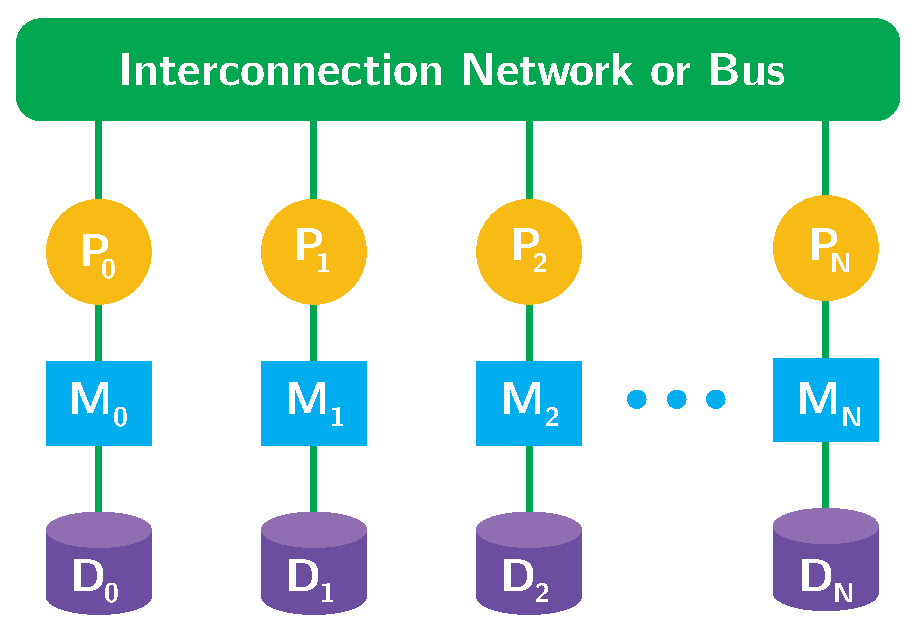
\includegraphics[width=0.45\textwidth]{ade_final_model}
    \vspace{-0.5em}
    \caption{\emph{Shared nothing parallel system.}}
    \label{fig:model}
    \vspace{-6em}
\end{wrapfigure}

\subsection{Data partitioning}
\noindent
There are many scheme for data partitioning: Vertical, horizontal (including Round-Robin, Hash, Value Range), duplicate. This data operation often requires the most of the network, since it sends out almost all the database. I will take an example to illustrate the cost of data partitioning.

\paragraph{Hash partitioning} Assuming the relational database is collected in parallel. Which means our database is distributed among all nodes. In this case, denote $r_c$ is the average ``correct'' rate of the data tuple, which means $r_c$ portion of the database is in its assigned node. The total communication cost for this scheme is:
$$
C_{\mbox{com}} = {R} \times (1 - r_c)
$$
where ${R}$ is the total size of the database. As we can see, under this scheme of hash partitioning, the number of PEs ($N$) plays a crucial role in communication cost. If the network has enough bandwidth, the communication cost is divided by $N$ times because of parallel messages sending. The communication cost also depends on random chances. On another perspective, the cost for I/O in this case is also ${R} \times (1 - r_c)$. However, in practice, the data rate of disk I/O is much larger than the data rate of the network (5Gbps vs. 1Gbps). Therefore, if we have a small number of PEs, then the communication cost is the major factor in this case. On the other hand, if we have a large number of PEs and a well-connected network, the disk I/O cost might become a bottle neck factor.

\subsection{Join operation}
\noindent
Join operation is one of the most intensively used operation in practice. In this analysis, I will consider distributed Sort-Merge Join and GRACE Hash Join. 

\paragraph{Sort-Merge Join} According to the lecture note \cite{lec1011}, the communication cost for parallel processing (ignoring pipeline effect) is:
$$
C_{\mbox{com}} = (2 - \frac{1}{N}) \times \{R\}
$$
$$
C_{\mbox{I/O}} = 6 \times (1 - \frac{1}{N}) \times |R|
$$
In this case, the communication cost becomes dominant as there are more processing elements. In the case of increasing $N$, the sort operation will be speed up, but the cost of sending data to the merge node is much higher.

\paragraph{GRACE Hash Join} In this scheme, the all-to-all communication cost is denoted as $\alpha$. For the sake of simplicity, I assume that each PE has enough space to hold $|R|/N$ and $|S|/N$. Because of this assumption, we can reduce the number of communications to the number of processing element $N$. For this case, network setup time is negligible. There are N phrases for the communication. The communication cost in this case is:
$$
\alpha = N \times \frac{|R| + |S|}{N} \times \mbox{ transfer rate}
$$
As we can see here, for GRACE Hash Join, the communication cost for the operation itself does not depend on the network. Therefore, in this case, the communication cost depends on the size of the relation itself and also it is largely affected by the setup time in case each PE does not have enough space to hold the relation.

\subsection{Aggregation}
The most common aggregation is the ``group-by'' operator. This operation is commonly used in Data Warehouse and MapReduce. The communication cost of this operation depends linearly on the number of PEs, since there is only $N-1$ data paths. Each PE performs aggregation locally and then sends the result to the result node. This communication situation is similar to ``select'' operation or data partitioning operation.

\subsection{Skew handling}
Skew handling is important for load-balancing in distributed hash join operations. As in lecture note about skew handling \cite{lec12}, here I will focus on the Fine Bucket Method. The total I/O cost for the Fine Bucket Method is:
$$
C_{\mbox{I/O}} = 5 \times \frac{|R| + |S|}{N}
$$
This estimation can also be considered as communication cost for the fine bucket method. As we can see here, the cost depends on the number of PEs. In this scheme, communication cost also depends linearly on the data size.

\subsection{Optimization}
The optimization problem for communication cost depends on each operation itself. Typically, communication cost depends on the amount of data sent. Therefore, if we can minimize the data sent, we can optimize the communication cost. One vivid example of this is the distributed hash join operations. By using hash function, we know exactly the destination of the data tuple, without broadcasting the data to all PEs.

%%%%%%%%%%%%%%%%%%%%%%%%%%%%%%%%%%%%%%%%%%%%%%%%%%%%%%%%%%%%%%


\section*{Question 3: RDBMS in the Cloud environment}
\setcounter{section}{1}

\textit{Discuss the role of RDBMS in the environment of Cloud (with consideration regarding RDF and XML databases).} 

\vspace{1.5em}
\noindent
\textbf{Answer:} 
\noindent
Relational databases are facilitated through Relational Database Management Systems (RDBMS), some examples are Oracle, SQL Server, MySQL, Sybase, etc. The data stored in RDBMS is structured, robust, and often the best combination of performance and scalability. According to \cite{doom}, the characteristic of RDBMS is defined as follow:
\begin{itemize}
    \setlength{\itemsep}{0cm}
    \setlength{\parskip}{0cm}
    \item Database contains tables, tables contains columns and rows, and rows are made up of column values. Rows within a table all have the same schema.
    \item The data model is well defined in advance. A schema is strongly typed and it has constraints and relationships that enforce data integrity.
    \item The data model is based on a ``natural'' representation of the data it contains, not on an application's functionality.
    \item The data model is normalized to remove data duplication. Normalization establishes table relationships. Relationships associate data between tables.
\end{itemize}
The recent trend for a database system is to use the Cloud, which is a form of distributed database system. The most common reason for this trend is the scalability of the Cloud framework. While RDBMS is scalable within a single node, it is not so trivial concerning a distributed environment. On the other hand, the database system nowadays must be flexible in term of application. In an organization, here are many applications and services need the support from the database. Due to the limitation of RDBMS in the Cloud environment, there are two rising database scheme: RDF (key-value) and XML database.
\paragraph{RDF} is defined by \cite{doom} as follow:
\begin{itemize}
    \setlength{\itemsep}{0cm}
    \setlength{\parskip}{0cm}
    \item Domain can initially be thought of like a table, but unlike a table you don't define any schema for a domain. A domain is bassically a bucket that you put them into. Items within a single domain can have differing schema.
    \item Items are identified by keys, and a given item can have a dynamic set of attributes attached to it.
    \item In some implementations, attributes are all of a string type. In other implementations, attributes have simple types that reflect code types, such as ints, string arrays, and lists.
    \item No relationship are explicitly defined between domains or within a given domain.
\end{itemize}
By its definition and characteristics, the RDF is more suitable for the clouds compare to RDBMS. Besides, it is natural fit with code, which means the data in the cloud can be used in many multimedia applications. On the other hand, lacking the integrity and structure compare to RDBMS make it difficult to maintain the database and limit analytic operations. In conclusion, RDF is best in the following scenarios: Data is heavily document-oriented, development is heavily object-oriented, need a cheap solution for data storage, and the foremost concern is scalability.

\paragraph{XML database} The is one emerging trend that is using XML and RDF together \cite{xml}. An XML document is a collection of data. If being considered as a ``database'' format, XML has some advantages. For example, it is self-describing, it can describe complex data structure (graph, tree). The characteristic of XML makes it a good fit with RDF in Cloud environment, especially for some Natural Language Processing and Machine Learning task.

In conclusion, RDBMS provides a robust, integrity database management system but its lack of distributed scalability makes it not a good fit for cloud computing. On the other hand, RDF and XML database, by nature a semi-structured database scheme, is a perfect fit for cloud computing if the users' foremost concern is scalability.
%%%%%%%%%%%%%%%%%%%%%%%%%%%%%%%%%%%%%%%%%%%%%%%%%%%%%%%%%%%%%%


\section*{Question 4: Most interesting technique in the course}
\setcounter{section}{1}

\textit{Choose a method or a technique which is most interesting to you during this course, and describe the reason why you select it.} 

\vspace{1.5em}
\noindent
\textbf{Answer:} 
\noindent
During the course, I think my favorite topics are the GRACE Hash Join method and the relational database cost estimation model ($|R| \mbox{ and } \{R\}$).
\paragraph{Cost model} provides a high-level view of the relational database operations. Using simple, straight forward analysis, this cost model can give a big overall picture of the local relational operations as well as distributed operations. The result of the analysis can be used to compare between methods, and give prediction on the expected behavior of the database system. 
\paragraph{GRACE Hash Join} is a fantastic method for join operation in general and distributed join operation in specific. By using the same hash partition function, all PEs can ``communicate'' instantly by mathematics. All data communication in this scheme is ``necessary'', which means there is minimized amount of excessive data communication. I believe this idea and technique can be further apply to many other researches in the future.


%%%%%%%%%%%%%%%%%%%%%%%%%%%%%%%%%%%%%%%%%%%%%%%%%%%%%%%%%%%%%%


\section*{Question 5: Course comment}
\setcounter{section}{1}

\textit{Write your comments on this course.} 

\vspace{1.5em}
\noindent
\textbf{Answer:} 
\noindent
I think this is a very informative course, and I enjoyed the process of studying database system. However, there are 2 minor points that I want to point out:
\begin{itemize}
    \setlength{\parskip}{0cm}
    \setlength{\itemsep}{0cm}
    \item There is no textbook or reference paper. I think it is necessary to have some reference textbooks or papers that are closely related to the course.
    \item The course can be more interesting if there is a project and demonstration in class (project based learning). Personally, I prefer working on a project to learning only theory.
\end{itemize}

\bibliography{ade_final}
\bibliographystyle{acm}

\end{document}
